\documentclass{beamer}
\usetheme{PaloAlto}
\usecolortheme{Crane}
\usepackage[utf8]{inputenc} 

\title[TDD] {Test Driven Development-menetelmän vaikutus laatuun ja taloudellisuuteen}
\author[] 
{Petri Pihlajaniemi}


\begin{document}
\frame{\titlepage}
%\begin{frame}
%\frametitle{Sisältö}
%\tableofcontents
%\end{frame}

\section{TDD}

\begin{frame}
    	\frametitle{Test Driven Development}
	\begin{itemize}
		\item Ohjelmistokehityksen menetelmä jossa testit kirjoitetaan ensin. Vertaa vesiputousmalliin.
		\item Kent Beck, 2002, Test Driven Development: By Example. 
		\item Myös Test First Development tai testivetoinen kehitys.
	\end{itemize}
\end{frame}


\subsection{Menetelmä}

\begin{frame}
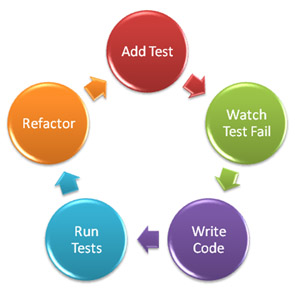
\includegraphics[width=4cm,height=4cm]{tddcycle.jpg}
	\frametitle{TDD:n prosessi}
	\begin{enumerate}
	\item Luodaan testi.
	\item Yritetään ajaa testit
	\item Kirjoitetaan koodia
	\item Ajetaan testit.
	\item Siistitään koodi.
	\end{enumerate}
\end{frame}

\subsection{Hyvää ja  huonoa}

\begin{frame}
    	\frametitle{Hyvää ja huonoa}
 Hyvää
	\begin{itemize}
	\item Takaa testien koodikattavuuden
	\item Helpommin ylläpidettävä ja laajennettava rakenne
	\item Virheet havaitaan aiemmin.
	\end{itemize}
Huonoa
	\begin{itemize}
	\item Paljon testikoodia
	\item Hyvien testien kirjoittamien vaikeaa
	\item Hankala käyttää tietyissä tehtävissä tai ympäristöissä


	\end{itemize}
\end{frame}



\section{Laatu}
\begin{frame}
    	\frametitle{Laatu}
	\begin{itemize}
	\item Useita erilaisia laatumalleja.
	\item Laatu riippuu myös näkökulmasta: käyttäjä, ohjelmoija...
	\item Kitchenham ja Pfleegerin näkökulmat
		\begin{itemize}
		\item Trancendental, User, Manufacturing, Product, Value
		\end{itemize}
	\item Suosittu laatumalli ISO 9126.
	\end{itemize}
\end{frame}

\subsection{ISO-standardi}
\begin{frame}
    	\frametitle{ISO9126}
	\begin{itemize}
	\item Suosittu laatumalli, ensimmäinen versio vuonna 1991. Uudempi ISO 25010 ei ole vielä syrjäyttänyt.
	\item Laatu koostuu osista jotka vaikuttavat toisiinsa
		\begin{itemize}
		\item Sisäinen laatu
		\item Ulkoinen laatu
		\item Käyttölaatu
		\end{itemize}
	\end{itemize}

\end{frame}

\begin{frame}
    	\frametitle{ISO9126}
	\begin{itemize}
	\item Standardin laatumallin kriteerit
		\begin{itemize}
		\item Toimivuus
		\item Luotettavuus
		\item Käytettävyys
		\item Tehokkuus
		\item Ylläpidettävyys
		\item Siirrettävyys
		\end{itemize}
	\item TDD:n vaikutuksia on vaikea asettaa luokkiin.
	\end{itemize}
\end{frame}

\section{Taloudellisuus}

\begin{frame}
    	\frametitle{Taloudellisuus}
	\begin{itemize}
	\item Efficiency = taloudellinen tehokkuus.
	\item Effectiveness = tehokkuus.
	\item Joskus epäselvää kumpaa artikkeleissa tarkoitetaan.
	\item Taloudellisuutta usein mitattu testien ja virheiden määrällä verrattuna käytettyyn vaivaan.
	\end{itemize}
\end{frame}

\section{Tutkimuksia}

\begin{frame}
    	\frametitle{Tutkimuksia}
	\begin{itemize}
	\item TDD:n vaikuksesta löytyy tutkimustietoa. Esim. Rafique ja kumppanit vertailleet 27 empiiristä tutkimusta.
	\item Mielestäni haasteellinen tutkimusalue, erilaisia ohjelmia, ohjelmoijia ja mittaustapoja. 
	\end{itemize}

\end{frame}

\subsection{Keilailukata}

\begin{frame}
    	\frametitle{Keilailukata}
	\begin{itemize}
	\item Keilailun pistelaskun toteutus on tunnettu ohjelmointiharjoitus. Robert Martin, Agile Manifesto
	\item Erdogmus et al ja Causevic et al tutkivat aihetta hyvin samankaltaisin menetelmin.
	\item Molemmissa vaikutus laatuun oli pieni. Tehokkuus 
	\end{itemize}

\includegraphics[width=2cm,height=2cm]{keilat.png}

\end{frame}

\begin{frame}
    	\frametitle{Keilailukata 2}
	\begin{itemize}
	\item George ja Williams tutkivat myös keilausta, pienin muutoksin verrattuna edellisiin.
		\begin{itemize}
		\item Ammattilaisia kolmesta yrityksestä
		\item Pariohjelmointi
		\end{itemize}
	\item TDD:tä käyttäneet läpäisivät 18\% enemmän testejä, mutta käyttivät 16\% enemmän aikaa.

	\end{itemize}

\end{frame}

\begin{frame}
    	\frametitle{Mitä tulokset tarkoittavat?}
	\begin{itemize}
	\item Tulokset eivät olleet kovin vahvoja
		\begin{itemize}
		\item Huonosti soveltuva ohjelma?
		\item Liian pieniä ja vääriä testiryhmiä?
	 	\item TDD ei toimi?
		\end{itemize}
	\item Tarvitaan useiden tutkimusten meta-analyysia.
	\end{itemize}

\end{frame}

\subsection{Rafique}
\begin{frame}
    	\frametitle{Rafiquen analyysi}
	\begin{itemize}
	\item Rafiquen ja kumppanien meta-analyysin mukaan:
			\begin{itemize}
		\item Pieni positiivinen vaikutus laatuun, mutta ei havaittavaa vaikutusta tuottavuuteen.
		\item Akateemisilla testiryhmillä positiivinen vaikutus laatuun oli selvästi pienempi kuin ammattilaisilla.
		\item Toisaalta ammattilaisilla tuottavuus putosi 

		\end{itemize}

	\end{itemize}

\end{frame}

\section{Yhteenveto}

\begin{frame}
	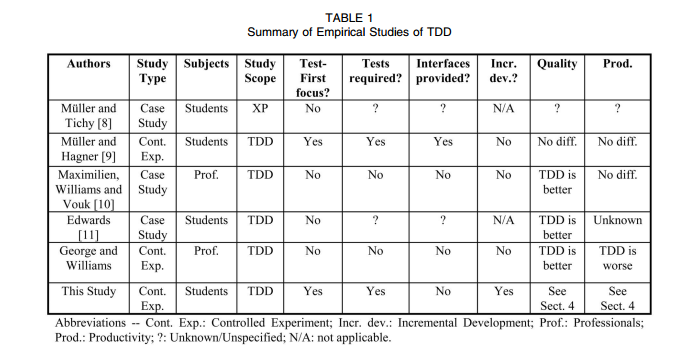
\includegraphics[width=10cm,height=5cm]{table.png}
    	\frametitle{Yhteenveto}
	\begin{itemize}
	\item Parantaako TDD laatua?
		\begin{itemize}
		\item Parantaa, mutta vaikutus on pieni.
		\end{itemize}
	\item Parantaako TDD taloudellisuutta?
		\begin{itemize}
		\item Vaikutus on neutraali.
		\end{itemize}
		

	\end{itemize}

\end{frame}

\begin{frame}
    	\frametitle{Kysyttävää?}
	\begin{itemize}
	\item Vastaan parhaani mukaan...

	\end{itemize}

\end{frame}










\end{document}